\documentclass[pdf]{beamer}

\usetheme{Boadilla}

\usepackage{amsmath}
\usepackage{amssymb}
\usepackage{tikz}

\logo{
    \begin{tikzpicture}[overlay,remember picture]
        \node[left=0.2cm] at (current page.34){
        
\includegraphics[width=1cm]{BYU_Cougars_logo.png}
};
    \end{tikzpicture}
}

\setbeamertemplate{footline}
{
  \leavevmode
  \hbox{
  \begin{beamercolorbox}[wd=.333333\paperwidth,ht=2.25ex,dp=1ex,center]{author in head/foot}%
    % \usebeamerfont{author in head/foot}\insertshortauthor
  \end{beamercolorbox}
  \begin{beamercolorbox}[wd=.333333\paperwidth,ht=2.25ex,dp=1ex,center]{title in head/foot}%
    \usebeamerfont{title in head/foot}\insertshorttitle
  \end{beamercolorbox}
  \begin{beamercolorbox}[wd=.333333\paperwidth,ht=2.25ex,dp=1ex,right]{date in head/foot}%
    % \usebeamerfont{date in head/foot}\insertshortdate{}\hspace*{2em}
    \insertframenumber{} / \inserttotalframenumber\hspace*{2ex} 
  \end{beamercolorbox}}
  \vskip0pt
}

\mode<presentation>{}

\title{TDA Review}
\institute{Brigham Young University}
\author{Tyler Trogden}
\date{\today}

\begin{document}
    \begin{frame}
        \titlepage
    \end{frame}

    \begin{frame}{Math Basics}
        \newtheorem{defn:inj}{Injective}
        \newtheorem{defn:surj}{Surjective}
        \newtheorem{defn:bi}{Bijective}
        \newtheorem{defn:preim}{Pre-image}

        \begin{defn:inj}
            A function $f: X \to Y$ is injective if $f(x_1) = f(x_2)$ implies $x_1 = x_2$.
        \end{defn:inj}
        \begin{defn:surj}
            A function $f: X \to Y$ is surjective if $y \in Y$ implies there exists $x \in X$ such that $f(x) = y$.
        \end{defn:surj}
        \begin{defn:bi}
            A function $f: X \to Y$ is bijective if it is both injective and surjective.
            (Equivalently $f$ is bijective if $f$ has both a left and right inverse.)
        \end{defn:bi}
        \begin{defn:preim}
            The pre-image of $y \in Y$ under $f: X \to Y$ is the set of all $x \in X$ such
            that $f(x) = y$. This can be extended to whole subsets of $Y$ by letting the
            pre-image of $U \subseteq Y$ be the set of all $x \in X$ such that $f(x) \in U$.
        \end{defn:preim}

    \end{frame}

    \begin{frame}{Topology}
        Let $X$ be a set. A {\color{red} topology} $\tau$ on $X$ is a collection of subsets of $X$
        called open sets such that:

        \begin{enumerate}
            \item $\emptyset, X \in \tau$,
            \item the union of an arbitrary collection of subsets of $\tau$ is in $\tau$, and
            \item the intersection of a finite collection of subsets of $\tau$ is in $\tau$.
        \end{enumerate}

        We call $(X, \tau)$ a topological space. \\~\\

        We could have just as easily defined a topology in terms of closed sets. However, the 
        relationship between open and closed sets of a topological space is easy enough. Let 
        $C \subseteq X$, if $X - C \in \tau$, then $C$ is closed.

    \end{frame}

    \begin{frame}{Topology}
        \framesubtitle{Bases Lemmas}
        \newtheorem{lemma:13.1}{Lemma 13.1 in Munkres}
        \newtheorem{lemma:13.2}{Lemma 13.2 in Munkres}

        A {\color{red} basis} $\mathcal{B}$ of $\tau$ is a collection of subsets of $X$ such that:

        \begin{enumerate}
            \item for every $x \in X$, there is at least one $B \in \mathcal{B}$ such that $x \in B$, and
            \item if $x \in X$ belongs to the intersection of $\{B_1, \hdots, B_n \} \subseteq \mathcal{B}$, 
                  then there exists $B \in \mathcal{B}$ such that $B = \bigcap_{i = 1}^n B_i$, where $x \in B$.
        \end{enumerate}

        \begin{lemma:13.1}
            Let $(X, \tau)$ be a topological space. Let $\mathcal{B}$ be a basis of $\tau$
            on $X$. Then for every $U \in \tau$ there exists a collection of basis elements
            $\{B_\alpha\}_{\alpha \in J}$ such that $U = \bigcup_{\alpha \in J} B_\alpha$.
        \end{lemma:13.1}
        \begin{lemma:13.2}
            Let $(X, \tau)$ be a topological space. Suppose there exists a collection
            of open sets $\mathcal{C} $ such that for every open set $U$ of $X$ and 
            every $x \in U$, there exists $C \in \mathcal{C}$ such that $x \in C$. Then
            $\mathcal{C}$ is a basis of $\tau$.
        \end{lemma:13.2}

    \end{frame}

    \begin{frame}{Topology}
        \framesubtitle{Limit Points}
        \newtheorem{cor:17.7}{Corollary 17.7 in Munkres}

        Let $(X, \tau)$ be a topological space. A point $x \in X$ is a {\color{red} limit point}
        of a subset $A \subseteq X$ if every neighborhood of $x$ contains a point of $A$. Here 
        we say that a neighborhood of $x$ is a set $N$ such that $x \in N$ and $N \in \tau$. \\~\\

        \begin{cor:17.7}
            A subspace of a topological space is closed if and only if it contains all of its limit points.
        \end{cor:17.7}

    \end{frame}

    \begin{frame}{Topology}
        \framesubtitle{Hausdorff Spaces}
        \newtheorem{thrm:conv}{Theorem 17.10 in Munkres}

        A topological space $(X, \tau)$ is {\color{red} Hausdorff} if for every $x, y \in X$,
        $x \neq y$ implies that $x$ and $y$ have disjoint neighborhoods. \\~\\

        This definition says something about the separability of a topological space. Interestingly,
        it means that elements of a Hausdorff space are distinct. Especially considering limit 
        points of certain sequences. \\~\\

        The $T_1$ axiom is a weaker version of the Hausdorff axiom that says that every
        finite set is closed. \\~\\

        \begin{thrm:conv}
            If $X$ is Hausdorff, then a sequence $\{x_n\}$ in $X$ converges to at most one $x \in X$.
        \end{thrm:conv}

    \end{frame}

    \begin{frame}{Continuos Functions}
        \newtheorem{thrm:cont}{Theorem 18.1 in Munkres}

        A function $f: X \to Y$ is {\color{red} continuous} if for every open subset $V \subseteq Y$,
        the subset $f^{\text{pre}}(V) \subseteq X$ is open. \\~\\

        \begin{thrm:cont}
            Let $(X, \tau_X)$ and $(Y, \tau_Y)$ be topological spaces; let $f: X \to Y$. Then the following
            are equivalent:
            \begin{enumerate}
                \item $f$ is continuous,
                \item for every subset $A \subseteq X$, $f(\overline{A}) \subset \overline{f(A)}$,
                \item for every closed subset $C \subseteq Y$, the set $f^{\text{pre}}(C)$ is closed, and
                \item for each $x \in X$ and neighborhood $V$ of $f(x)$, there exists a neighborhood $U$ of $x$
                      such that $f(U) \subset V$.
            \end{enumerate}
        \end{thrm:cont}
        
    \end{frame}

    \begin{frame}{Continuos Functions}
        \framesubtitle{Homeomorphisms}
        
        Let $(X, \tau_X)$ and $(Y, \tau_Y)$ be topological spaces. A bijection $f: X \to Y$ is a 
        {\color{red} homeomorphism} if $f$ is continuous and $f^{-1}$ is continuous. (Note that 
        since $f$ is a bijection, $f^{-1}$ always exists.) \\~\\

        This can be restated in terms of open sets as follows: let $f$ be a bijection such that 
        $f(U)$ is open if and only if $U$ is open. Then $f$ is a homeomorphism. \\~\\

        Having a one-to-one correspondence between open sets gives us a way to map the topology
        of one space to the topology of another. Therefore, for any property of $X$ that is characterized
        entirely by the topoloy of $X$, the same property holds for $Y$ if $f$ is a homeomorphism. This
        property is then called a {\color{red} topological property}. \\~\\
        
    \end{frame}

    \begin{frame}{Metric Topology}
        
        A {\color{red} metric space} is a set $X$ together with a function $d: X \times X \to \mathbb{R}$
        satisfying the following conditions:
        \begin{enumerate}
            \item $d(x, y) \geq 0$ for all $x, y \in X$,
            \item $d(x, y) = 0$ if and only if $x = y$,
            \item $d(x, y) = d(y, x)$ for all $x, y \in X$,
            \item $d(x, y) \leq d(x, z) + d(z, y)$ for all $x, y, z \in X$.
        \end{enumerate}
        The function $d$ is called a {\color{red} metric} on $X$. \\~\\

        Let $(X, d)$ be a metric space. Given $\epsilon > 0$ the set 

        \[
            B_\epsilon(x) = \{y \in X \,|\, d(x, y) < \epsilon\}    
        \]

        is called the {\color{red} $\epsilon$-ball} centered at $x$. \\~\\

        A basis for a topology on $X$ is the collection of all $B_\epsilon(x)$
        for every $\epsilon > 0$ and $x \in X$. This topology is known as the 
        {\color{red} metric topology} induced by $d$. \\~\\
        
    \end{frame}

    \begin{frame}{Metric Topology}
        \framesubtitle{Metrizability}
        \newtheorem{thrm:urysohn}{Urysohn Metrization Theorem}

        A topological space $(X, \tau)$ is {\color{red} metrizable} if there exists a metric $d$ on $X$
        that induces the topology of $X$. A metric space is a metrizable space $X$ together with a
        specific metric $d$ that gives the topology of $X$. \\~\\

        Having a metrizable topological space is useful because it allows us to use the metric
        in order to prove certain theorems in topology. Therefore, we'd like to be able to show
        that a given topological space is metrizable. This is where the {\color{red} Urysohn 
        Metrization Theorem} comes in (among others). \\~\\

        \begin{thrm:urysohn}
            Every regular space $X$ with a countable basis is metrizable.
        \end{thrm:urysohn}

        A space is {\color{red} regular} if for each pair consisting of a point $x$ and a closed set
        $C$ not containing $x$, there exists disjoint neighborhoods containing $x$ and $C$ respectively.

    \end{frame}

    \begin{frame}{Connectedness and Compactness}
        \framesubtitle{Connectedness}

        Let $(X, \tau)$ be a topological space. A {\color{red} separation} of $X$ is a pair of disjoint
        non-empty open sets $U, V \subseteq X$ whose union is $X$. A space is {\color{red} connected} 
        if it has no separation. Connectedness is a topological property which is invariant. \\~\\

        Put differently a space $X$ is connected if and only if the only subsets of $X$ that are
        both open and closed in $X$ are $X$ and $\emptyset$. \\~\\
        
    \end{frame}

    \begin{frame}{Connectedness and Compactness}
        \framesubtitle{Connectedness Theorems}
        \newtheorem{thrm:entire}{Theorem 23.2 in Munkres}
        \newtheorem{thrm:closure}{Theorem 23.4 in Munkres}
        \newtheorem{thrm:image}{Theorem 23.5 in Munkres}

        Let $(X, \tau)$ be a topological space.

        \begin{thrm:entire}
            If sets $C$ and $D$ form a separation of $X$, and if $Y \subseteq X$ is connected, then
            $Y$ is either a subset of $C$ or a subset of $D$. \\~\\
        \end{thrm:entire}

        \begin{thrm:closure}
            Let $A \subseteq X$ be connected. If $A \subseteq B \subseteq \bar{A}$, then
            $B$ is also connected. \\~\\
        \end{thrm:closure}

        \begin{thrm:image}
            The image of a connected space under a continuous map is connected. \\~\\
        \end{thrm:image}

    \end{frame}

    \begin{frame}{Connectedness and Compactness}
        \framesubtitle{Compactness}

        A collection $\mathcal{C}$ of subsets of a topological space $(X, \tau)$ covers
        $X$ if $\bigcup_{C \in \mathcal{C}} C = X$. It is said to be an {\color{red} open cover}
        if each $C \in \mathcal{C}$ is open. \\~\\

        A space $X$ is {\color{red} covering compact} if every open cover of $X$ has a finite subcover.
        From now on we shorten covering compact to simply compact. \\~\\
        
    \end{frame}

    \begin{frame}{Connectedness and Compactness}
        \framesubtitle{Compactness Theorems}
        \newtheorem{thrm:closedSub}{Theorem 26.2 in Munkres}
        \newtheorem{thrm:closedComp}{Theorem 26.3 in Munkres}
        \newtheorem{thrm:imageComp}{Theorem 26.5 in Munkres}

        \begin{thrm:closedSub}
            Every closed subspace of a compact space is compact. \\~\\
        \end{thrm:closedSub}

        \begin{thrm:closedComp}
            Every compact subspace of a Hausdorff space is closed. \\~\\
        \end{thrm:closedComp}

        \begin{thrm:imageComp}
            The image of a compact space under a continuous map is compact. \\~\\
        \end{thrm:imageComp}

    \end{frame}

    \begin{frame}{Limit Point Compactness}
        \newtheorem{thrm:seqComp}{Theorem 28.2 in Munkres}

        A topological space $(X, \tau)$ is {\color{red} limit point compact} if every
        infinite subset of $X$ has a limit point. Limit point compactness is a weaker
        property than compactness, but the two coincide if $X$ is metrizable. In fact
        compactness implies limit point compactness, but not the other way round. \\~\\

        The space $X$ is said to be {\color{red} sequentially compact} if every sequence
        of points in $X$ has a convergent subsequence. \\~\\

        \begin{thrm:seqComp}
            Let $X$ be metrizable. Then the following are equivalent:
            \begin{enumerate}
                \item $X$ is compact.
                \item $X$ is limit point compact.
                \item $X$ is sequentially compact.
            \end{enumerate}
        \end{thrm:seqComp}
        
    \end{frame}

    \begin{frame}{Abstract Topology}
        \framesubtitle{Homotopy}

        Let $(X, \tau)$ be a topological space. A {\color{red} homotopy} from $f: A \to X$ to $g: A \to X$,
        both continuos, is a continuous map $H: A \times [0, 1] \to X$ such that $H(a, 0)
        = f(a)$ and $H(a, 1) = g(a)$ for all $a \in A$. The homotopy $H$ is parametrized by 
        $t \in [0, 1]$, which may be thought of as time. Essentially $H$ represents a continuos
        deformation of $f$ into $g$. \\~\\

        Now suppose that we are considering two maps $f, f': [0, 1] \to X$ which happen
        to be paths in $X$ with the same initial point $x_0$ and final point $x_1$.
        If there exists a continuous map $P: [0, 1] \times [0, 1] \to X$ such that 

        $$
            P(s, 0) = f(s), \quad P(s, 1) = f'(s), \quad P(0, t) = x_0, \quad P(1, t) = x_1 \nonumber
        $$

        for every $s, t \in [0, 1]$, then we say that $f$ and $f'$ are {\color{red} homotopic}
        with $P$ being the {\color{red} path homotopy}. As Munkres says, ``the first condition
        says that $P$ represents a continuous way of deforming the path $f$ to the path
        $f'$, and the second condition says that the end points of the path remain fixed
        during the deformation.'' \\~\\

    \end{frame}

    \begin{frame}{Abstract Topology}
        \framesubtitle{Homotopy}

        It turns out that both homotopy and path homotopy form equivalence relations on their 
        respective sets of maps. For our purposes we will focus on path homotopy with its 
        equivalence relation denoted as $\simeq_p$ and its equivalence class denoted as $[f]$. \\~\\

        If $f$ is a path in $X$ with initial point $x_0$ and final point $x_1$, and if $f'$
        is another path in $X$ with initial point $x_1$ and final point $x_2$, we define the
        {\color{red} product} $f * f'$ to be the path $h$, which is defined  as

        $$h(s) =
        \begin{cases}
            f(2s) &, \text{if } 0 \leq s \leq \frac{1}{2} \\
            f'(2s - 1) &, \text{if } \frac{1}{2} \leq s \leq 1
        \end{cases}.
        $$

        Since $f$ and $f'$ are continuous paths in $X$, we know that $h$ is also a continuous path in $X$. \\~\\

    \end{frame}

    \begin{frame}{Abstract Topology}
        \framesubtitle{The Fundamental Group}

        The product operation $*$ may also be used to induce an operation on the set of equivalence
        classes of paths. Let $[f]$ and $[f']$ be two equivalence classes of paths in $X$, then
        we have $[f] * [f'] = [f * f']$. \\~\\

        The {\color{red} fundamental group} of a topological space $(X, \tau)$ is the set of equivalence
        classes of paths in $X$ with the $*$ operation. The fundamental group is denoted as $\pi_1(X, x_0)$
        where $x_0$ is a chosen fixed point in $X$. This fixed point is called the {\color{red} base point}
        and we consider only those paths which start and end at the base point. This way we guarantee that the fundamental group is indeed a group. \\~\\
        
    \end{frame}

    \begin{frame}{Topological Data Analysis}
        Topological data analysis, or TDA, is a relatively new field of mathematics which began as a branch 
        of algebraic topology. The goal of TDA is to extract information about a data set by using topological
        methods. The data set is usually a finite set of points in $\mathbb{R}^n$ with some notion of distance
        between points, however, we may also use more abstract sets as well. \\~\\

        The first step in TDA is to construct a simplicial complex from the data set. For our purposes we will
        be using abstract simplicial complexes which along with their geometric realizations form a topological
        space. We will then use the topological space to compute the homology groups of the simplicial complex
        at various scales.
    \end{frame}

    \begin{frame}{Topological Data Analysis}
        \framesubtitle{Simplicial Complexes}
        \newtheorem{defn:complex}{Abstract Simplicial Complex}

        \begin{defn:complex}
            An {\color{red} abstract simplicial complex} $K$ is a collection of finite sets that is closed under
            subsets.The sets $\sigma \in K$ are called {\color{red} simplices} and the subsets of $\sigma$ are 
            called {\color {red} faces}. The {\color{red} dimension} of a simplex $\sigma$ is one less than
            its cardinality. The {\color{red} dimension} of $K$ is the maximum dimension of any simplex in $K$. \\~\\
        \end{defn:complex}

        \begin{figure}
            \centering
            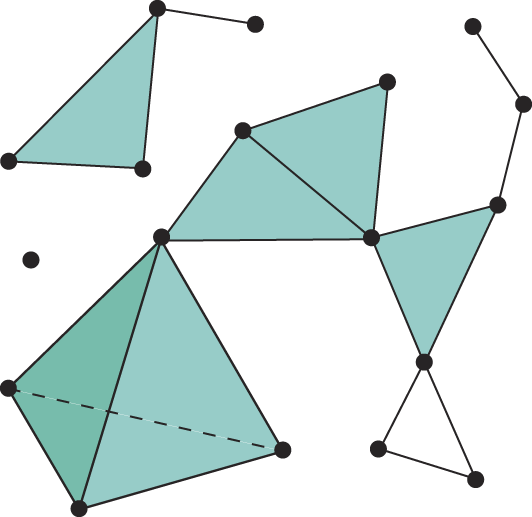
\includegraphics[scale=0.4]{simp_comp.png}
            \caption{A geometric realization of an abstract simplicial complex.}
        \end{figure}
    \end{frame}

    \begin{frame}{Topological Data Analysis}
        \framesubtitle{Chain Groups}
        \newtheorem{defn:chain}{Chain Group}

        \begin{defn:chain}
            Let $K$ be an abstract simplicial complex. The {\color{red} chain group} $C_p(K)$ is the free abelian group
            generated by the $p$-simplices of $K$. The elements of $C_p(K)$ are called {\color{red} $p$-chains}.
        \end{defn:chain}

        Elements of $C_p(K)$ are formal sums of $p$-simplices with coefficients over a field or ring. Most 
        often the coefficients are taken from $\mathbb{Z}_2$ in order to denote the presence or absence of a
        simplex in a chain. Further, elements of $C_p(K)$ are added component-wise. E.g., if $c$ and $c'$
        are $p$-chains such that $c = \sum_{i=1}^n a_i \sigma_i$ and $c' = \sum_{i=1}^n b_i \sigma_i$, then
        $c + c' = \sum_{i=1}^n (a_i + b_i) \sigma_i$. (Note that this is equivalent to the symmetric difference
        when using $\mathbb{Z}_2$ coefficients.)
    \end{frame}

    \begin{frame}{Topological Data Analysis}
        \framesubtitle{The Boundary Operator}
        \newtheorem{defn:bop}{Boundary Operator}

        \begin{defn:bop}
            Let $K$ be an abstract simplicial complex. The {\color{red} boundary operator} $\partial_p : C_p(K) \to C_{p-1}(K)$
            is the unique homomorphism such that $\partial_p(\sigma) = \sum_{i=0}^p (-1)^i \sigma_{[i]}$ for every
            $p$-simplex $\sigma$ in $K$.
        \end{defn:bop}

        The boundary operator is a linear map which gives us a way to move between the chain groups of different
        dimensions. The image of a chain group under the boundary operator is called the {\color{red} boundary group}.
        Similarly, the kernel of the boundary operator is called the {\color{red} cycle group}. \\~\\

        Formally, we have $B_p(K) = \text{im}(\partial_{p+1})$ and $Z_p(K) = \text{ker}(\partial_p)$.
    \end{frame}

    \begin{frame}{Topological Data Analysis}
        \framesubtitle{Homology}
        \newtheorem{defn:homology}{Homology Group}

        \begin{defn:homology}
            Let $K$ be an abstract simplicial complex. The {\color{red} $p$-th homology group} of $K$ is the quotient 
            group $H_p(K) = Z_p(K) / B_p(K)$ where $Z_p(K)$ is the $p$-th cycle group and $B_p(K)$ is the $p$-th 
            boundary group.
        \end{defn:homology}

        The homology groups of a simplicial complex are a topological invariant which give information about the 
        connected components, holes, tunnels, voids, etc. of the complex. The order/rank of the homology groups
        is given by 

        \begin{equation*}
            \text{rank}(H_p(K)) = \text{dim}(Z_p(K)) - \text{dim}(B_p(K)).
        \end{equation*}

        Further, the rank of the $p$-th homology group is the same as the number of $p$-dimensional holes in the complex, i.e., its $p$-dimensional {\color{red} Betti number} $\beta_p$.
    \end{frame}

\end{document}